\section{Generating Explanations with Concept Relevance Propagation}\label{section:explanations_with_crp}
The previously described causal framework can be applied to a multitude of explanation methods which have concept-specific attribution maps. However, we limit our analysis to CRP and interpretation techniques constructed with CRP. This is mostly due to the time limitations of a master thesis, but also because its authors specifically claim in their paper that CRP facilitates identifying relative importance. 
Producing explanations using CRP requires decisions on the backpropagation rules, on the conditioning sets and further hyperparameters. 
We follow the recommendations and default settings of CRP's authors \citep{Achtibat2022, Achtibat2023} and best practices \citep{Kohlbrenner2020} as closely as possible.
For the backpropagation we apply the $LRP_{\varepsilon -z^+- b^-}$ - rule as recommended by \cite{Kohlbrenner2020}. Due to the simplicity of our CNN model no more model canonization steps need to be applied. See \cref{appendix:lrprules} for further technical details. 

\begin{figure}[t!]
    \centering
    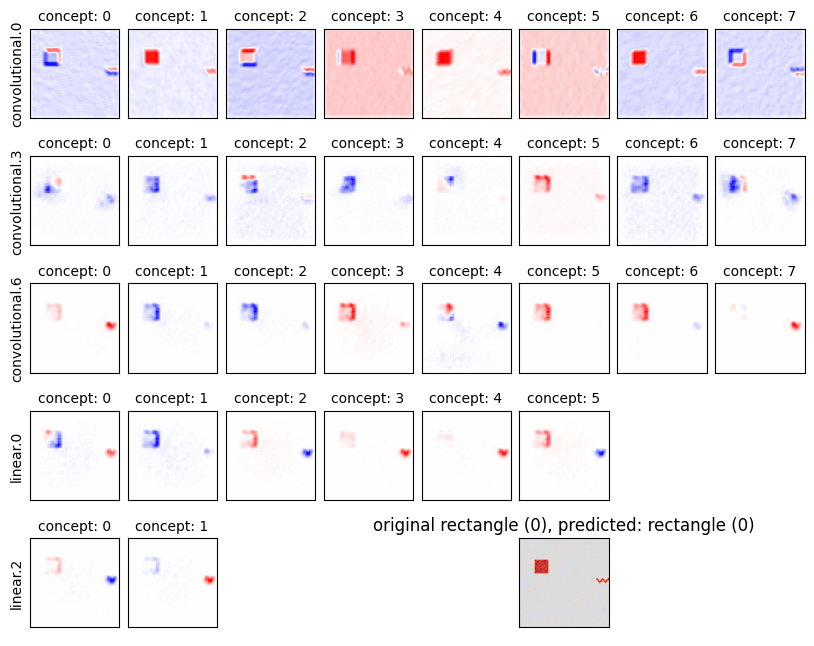
\includegraphics[width=0.8\textwidth]{thesis_latex_template/pics/conditional_heatmaps.png}
    \caption[Comparing Attribution Maps of Layers]{Concept-conditional heatmaps for one example image (rectangle with watermark) and each neuron within our small model. While the first convolutional layer's attributions are akin to edge detection filters (``convolutional.0'' in top row), later layers seem to encode more abstract concepts. For example, some only attribute the shape, some only the watermark, and others a combination of both.}
    \label{fig:cc_heatmaps}
\end{figure}

Principally, neurons in every layer of a model can be conditioned on using the CRP approach. However, the resulting attribution maps are not necessarily depicting disentangled \textit{and} abstract enough concepts. When looking at concept-conditional attribution maps from the earlier layers, one will likely see low-level features akin to edge detection filters. In the late, fully connected, layers before the output the previously disentangled concepts might get mixed together again for the final decision. In \cref{fig:cc_heatmaps} an example shows the tendency from trivial to abstract concepts. 
According to \cite{Dreyer2023a}, who refer to \cite{Zeiler2013}, the \textit{last convolutional layer} is ``most likely representing disentangled representation''. This is why we use the third and last convolutional layer of our minimal model for the analysis.  
Due to our principled approach, with many models to be trained, we opted for a compact architecture, which achieves perfect accuracy for the simple prediction task at hand and requires little computing time. The transferability of our results to large neural networks should be subject of further investigation.
In the following we will reiterate the steps necessary to produce different components of CRP-explanations in our experiment.

\subsubsection{Concept-Conditional Attribution Maps and Relevance for Prediction}
The concept-conditional backpropagation rule described in \cref{section:crp_background} can be applied to arbitrary sets of neurons $\theta$. In our scenario we create class-specific attribution maps conditioned on each individual neuron (termed concept $c$) in the selected layer. For this, we use the output as the initialization for relevance, keep all other layers untouched and then mask out the desired neuron's relevance in the layer $\ell$: 
\begin{equation}
    R^{\ell}_{c}(\mathrm{x} |\theta_{c}) = \sum_{i} R_i^{\ell}(\mathrm{x} |y \cup \theta_{\ell} = \{c\})
\end{equation}
Here $i$ represent all relevances in lower layers that are a part of the concept $c$ and not masked out. 
To yield the attribution map, the importance is back-propagated through all layers until the input layer $\ell = 1$, producing pixel-wise relevances conditioned on concept $c$, termed $R_{i}^{1}(\mathrm{x} |\theta_{c})$. In the following we will refer to this concept-conditional attribution map as $\mathcal{A}_c(\mathrm{x})$ and the class specific relevance of concept $c$ as $R_c^{\ell}(\mathrm{x})$. Due to the \textit{conservation laws} that CRP inherits from LRP (compare Equation 7, \cite{Achtibat2022}) the relevances $R_c^{\ell}$ within one layer can be interpreted as the \textit{percentage} of importance going through concept $c$. To enable this view also for out-of-distribution samples the authors recommend normalizing the relevances to sum to 1, by dividing through the absolute sum of relevance:
\begin{align}\label{eq:normed_relevance}
    R^{\ell}_{c,norm}(\mathrm{x} |\theta_{c}) = \frac{R^{\ell}(\mathrm{x} |\theta_{c}) }{\sum_k |R_k^{\ell}(\mathrm{x} |\theta_{c})|}.
\end{align}

\subsubsection{Local Concept Importance}
To find out how much a certain region contributes to the overall prediction but also which concepts are most highly activated within that region, the authors propose local concept importance. 
This method simply masks out the desired region (or input pixels), within the concept-conditional attribution map and sums the relevance within that mask. 
For readability we from now on refer to this local concept importance in a region $B$ as $R_B$.

\begin{align}\label{eq:local_importance}
    R_{B}^{\ell}(\mathrm{x} | \theta_c) = \sum_{(p,q) \in B} R_{p,q}^{\ell}(\mathrm{x} | \theta_c)
\end{align}

\subsubsection{Relevance Maximization}
As described in the background \cref{section:crp_background}, CRP's authors also use concept-conditional relevance to create prototypical reference sets of each concept. In a human subject study \citep{Achtibat2023} they find this method to be useful for the identification of Clever-Hans artifacts, where only using heatmaps is less useful. We therefore aim to include this technique into our analysis. The reference sets consist of images with maximal relevance for a neuron. Each image can be further concentrated on the encoded concept by thresholding the relevance and by cropping to the receptive field of the neuron in question. This yields a set of cropped images which ought to describe the encoded concept. 

As mentioned by \citet{Achtibat2022}, using the whole dataset might make the selected images too similar to each other. Hence, we compute the maximization for a subset of only 300 images to enforce more variance. This is especially necessary for the dSprites dataset because the difference between images is small. Importantly, the sample we select from does not have an association between $S$ and $W$, meaning that watermarks (or blurry patterns) are equally likely to occur on rectangle as on ellipse images. 
The provided implementation produces sets of 40 images for each neuron in each layer with either relevance or activation maximized using the sum or maximum (conditional) relevance/activation for an image. We mainly use the default option of maximizing for the sum of relevance of an image for a concept, but also look at the results when the maximization target is the maximal relevance of an image or when activation is used instead of relevance. Furthermore we use only the 15 top images, to emulate how these reference sets might be applied in real scenarios. 
The implementation of all previously described methods is made accessible by CRP's authors at
\url{https://github.com/rachtibat/zennit-crp}. 

Relevance maximization reference sets are denoted the following way:
 \begin{align}
\mathcal{T}_{sum}^{rel} (\mathrm{x}) & = \sum_{i} R_i(\mathrm{x}|\theta=\{c\}) \label{eq:rel_sum}\\
\mathcal{T}_{max}^{rel} (\mathrm{x}) & = \max_{i} R_i(\mathrm{x}|\theta=\{c\}) \label{eq:rel_max}\\
\mathcal{X}^{\star} & = \{ \mathrm{x}_{1}^{\star},\mathrm{x}_{2}^{\star},..., \mathrm{x}_{n}^{\star} \} = arg \sort_{\mathrm{x} \in \mathcal{X}} \mathcal{T}(\mathrm{x}) \\
\mathcal{X}_{k}^{\star} & = \{ \mathrm{x}_{1}^{\star},\mathrm{x}_{2}^{\star},..., \mathrm{x}_{k}^{\star} \} \subseteq \mathcal{X}^{\star}
 \end{align}

 \Cref{eq:rel_sum,eq:rel_max} describe the targets $\mathcal{T}$ to maximize when using either the sum or the maximum of relevance within an image. $\mathcal{X}_k^\star$ are then the top $k$ images when using target $\star$.